\documentclass{beamer}
\usetheme{Singapore}
\usecolortheme{default}

\usepackage[utf8]{inputenc}
\usepackage[T1]{fontenc}
\usepackage{verbatim}
\usepackage{graphics}
\usepackage{listings}
\usepackage{lmodern}

\title{Understanding Git with Alloy}
\subtitle{Milestone 1}
\author{Cláudio Lourenço \and Renato Neves}
\institute{University of Minho\\
Formal Methods in Software Engineering}


\logo{ 
\includegraphics[width=0.15\textwidth]{images/csail_logo.png}
       
\includegraphics[width=0.15\textwidth]{images/uminho_eng_logo.png}}

\begin{document}

\frame {
   \titlepage
}

\frame{
   \frametitle{Table of contents}
   \tableofcontents 
}
\section{Version Control System}
\frame{
   \frametitle{Version Control System}
         \begin{block}{What is a VCS?}
            \begin{itemize}
               \item Records changes on files over time  %progit 2.1 
               \item Recall old versions of files
            \end{itemize}
         \end{block}
         \begin{block}{Local VCS}
            No collaboration with other users - RCS %Revision Control System
         \end{block}
         \begin{block}{Centralized VCS}
            \begin{columns}[c]
               \column{3in}
               All files are stored on a central server - CVS, Subversion, Perfomance
               \column{1in}
                  \begin{figure}
                     
\includegraphics[width=0.4\textwidth]{images/centralized.png}
                  \end{figure}
            \end{columns}
         \end{block}
         \begin{block}{Distributed VCS}
            Each client has a mirror of the repository - Git, BitKeeper, Mercurial, Bazaar, Darcs%progit 2.1.3
         \end{block}
         \begin{figure}
            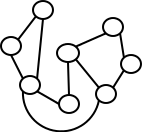
\includegraphics[width=0.1\textwidth]{images/distributed.png}
         \end{figure}
         
}

\section{Git in a nutshell}
\frame{
   \frametitle{Git in a nutshel}
      \begin{itemize}
         \item It was created in 2005 by Linus Torvalds
         \item Distributed Version Control System
         \item Simple, Fast, Efficient
         \item It keeps snapshots, not differences
         \item Operations with branches are very cheap
      \end{itemize}

}

\frame{
   \frametitle{Git simplified workflow }
   \begin{figure}
      \centering
      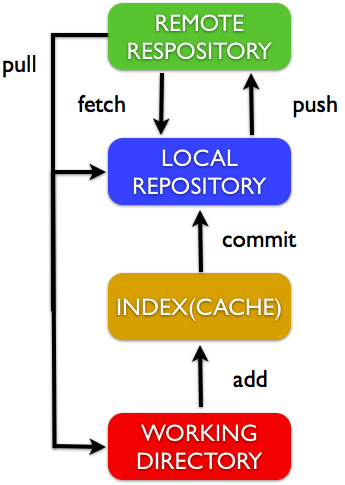
\includegraphics[width=0.35\textwidth]{images/data_flow_simplified.png}
   \end{figure}
   
}

\frame{
   \frametitle{The Git Object Model}
   \begin{columns}[c]
      \column{2in}
      \begin{itemize}
         \item Similar to a filesystem
         \item Each git object is named by a sha
         \item Blob stores the content of a file
         \item Tree references a set of others trees and blobs
         \item Commit points to a single tree
         \item Commit can have more than one parent 
      \end{itemize}
      \column{2in}
      \begin{figure}
         \centering
         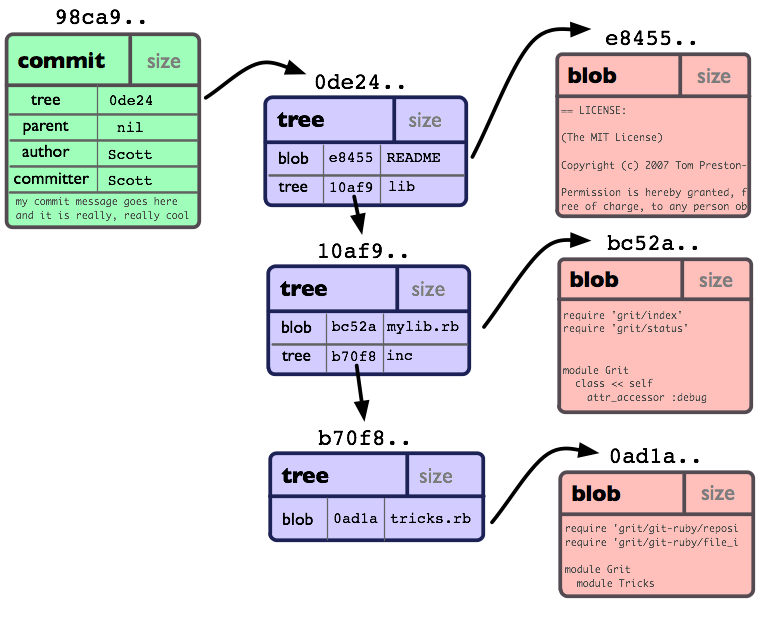
\includegraphics[width=1\textwidth]{images/object_model.png}
      \end{figure}
   \end{columns}
}


\section{Project Goals}
\frame{
   \frametitle{Project Goals}
   \begin{itemize}
      \item Build a precise model of how Git works
      \item Analyze the model
      \item Check which properties the model does (not) guarantee
      \item Compare to other systems
      \item Build a concise user manual based on the model
   \end{itemize}
}

\section{Progress so far}
\frame{
   \frametitle{What has been done so far}
   \begin{block}{First Approach}
      \begin{itemize}
         \item Model Working Directory
         \item Model Index
         \item Model Object Model
         \begin{itemize}
            \item Object's hash is modeled implicitly
         \end{itemize}
      \end{itemize}
   \end{block}
}


\begin{frame}[fragile]
   \frametitle{First Approach - Object Model}
   \tiny
   \begin{columns}[c]
      \column{1.5in}
   \begin{lstlisting}[escapechar=!]
sig Sha{}
sig State{}
   
abstract sig Object {
   namedBy : Sha one -> State
}

sig Blob extends Object{
   blobs: set State
}

sig Tree extends Object {
   references:(Tree+Blob) some-> State,
   trees: set State
}

sig Commit extends Object{
   points : Tree one -> State,
   parent : Commit set -> State,
   commits: set State
}

sig RootCommit extends Commit{}

   \end{lstlisting}
      \column{1.5in}
   \color{blue}{
   \begin{lstlisting}[escapechar=!]
   abstract sig WDObject{
      wdparent: Dir lone -> State,
      wdobjects: set State
   }

   sig File extends WDObject{
      content: Sha lone-> State
   }

   sig Dir extends WDObject{}

   one sig Root extends Dir{}
   \end{lstlisting}
   }
   \color{brown}{
   \begin{lstlisting}
   one sig Index{
      stage: Sha lone-> File -> State,
      indexes: set State
   }
   \end{lstlisting}
   
   }
   \end{columns}
\end{frame}

\begin{frame}[fragile]
   \frametitle{First Approach - Problems}
      \begin{itemize}
         \item Model got too complex when adding operations
         \item We need the name of the files and directories
         \item Some relations are not dynamic
      \end{itemize}
\end{frame}

\frame{
   \frametitle{What has been done so far}
   \begin{block}{Second Approach}
      \begin{itemize}
         \item Focus on the Object Model and Index
         \item Files are associated with a path and a blob
         \item Object hash are the alloy atom's name
      \end{itemize}

   \end{block}
}

\begin{frame}[fragile]
   \frametitle{Second Approach - Object Model}
   \tiny
   \begin{columns}[c]
      \column{1.5in}
   \begin{lstlisting}
sig Name {}
sig State {}

abstract sig Object {
   objects: set State
}

sig Blob extends Object {}

sig Tree extends Object {
   contains: Name -> one(Tree+Blob)
}

sig RootCommit extends Commit {}

sig Commit extends Object {
   points: one Tree,
   parent: set Commit
}

\end{lstlisting}
   \column{1.5in}
\color{brown}{
\begin{lstlisting}
sig Path {
   pathparent: lone Path,
   name: Name,
   blob:lone Blob,
   index: set State
}
   \end{lstlisting}
   }
   \end{columns}

\end{frame}

\frame{
   \frametitle{Instance - A single commit corresponding to an index}
   \begin{figure}
      \centering
      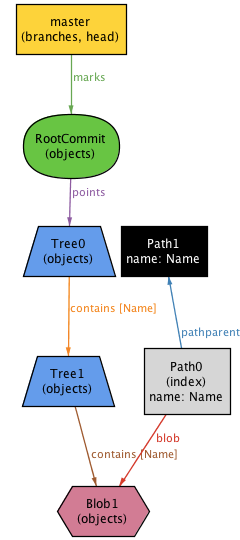
\includegraphics[width=0.30\textwidth]{images/commit_index.png}
   \end{figure}
}


\frame{
   \frametitle{Instance - Commits sharing objects}
   \begin{figure}
      \centering
      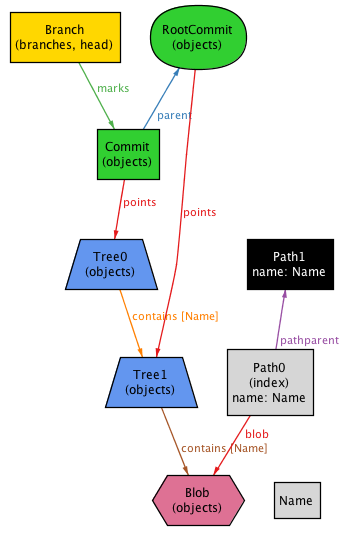
\includegraphics[width=0.4\textwidth]{images/commits_sharing.png}
   \end{figure}
}

\frame{
   \frametitle{Problems we are facing}
   \begin{figure}
      \centering
      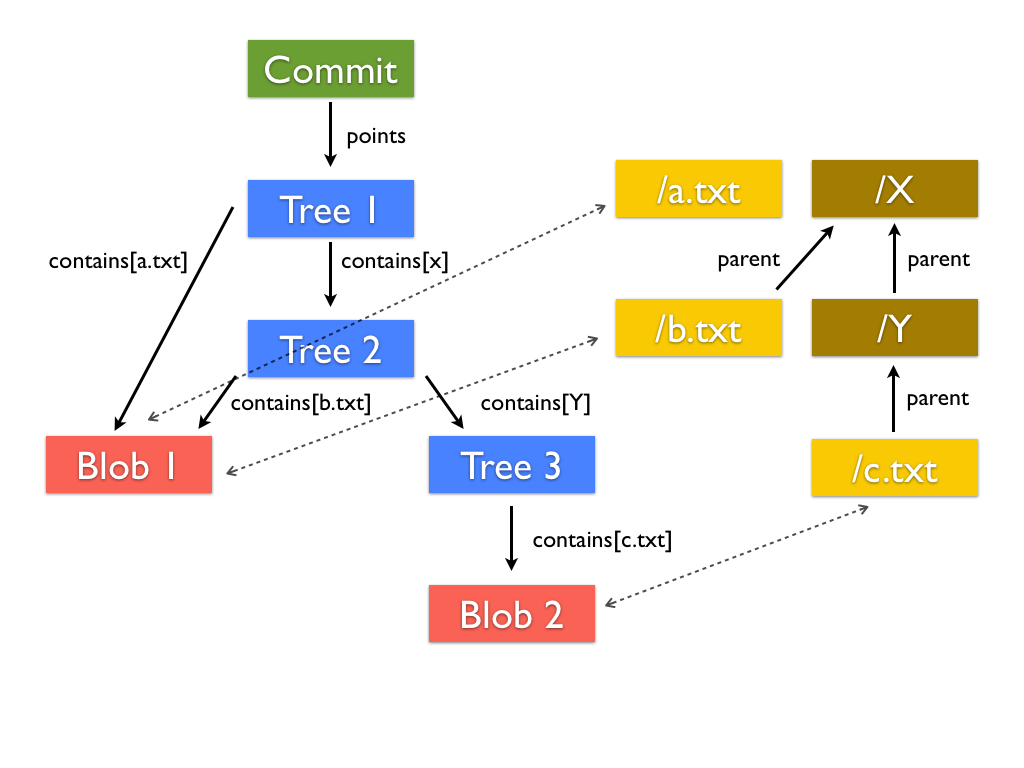
\includegraphics[width=0.9\textwidth]{images/structures.png}
   \end{figure}
}

\begin{frame}[fragile]
   \frametitle{Possible Solution}
      \footnotesize
      \begin{lstlisting}[escapechar=!]
      sig Commit extends Object {
         points : one Tree,
         parent : set Commit,
         !\color{red}{abs: Object lone -> some Path}!
     }
     \end{lstlisting}
\end{frame}

\section{Future Work}
\frame{
   \frametitle{Future work on the model}
   \begin{itemize}
      \item Find a solution for the current problem (Suggestions?)
      \item Model some operations relatively to the remote repository
      \item Analyze model and check some properties
   \end{itemize}
}

\frame{
   \titlepage
}


\end{document}
